\section{Programiranje soketa}

Za programiranje soketa u Pajtonu, možemo da koristimo ugrađenu soket biblioteku koja sadrži sve potrebne funkcije i klase koje su nam potrebne da pravimo i upravljamo soketima. Neke od češće korišćenih funkcija biblioteke su:
\begin{itemize}
    \item \textbf{socket():} Pravi novi soket;
    \item \textbf{bind():} Asocira soket sa specifičnom adresom i portom;
    \item \textbf{listen():} Započinje slušanje za dolazne veze na soketu;
    \item \textbf{accept():} Prihvata zahtev za vezu od strane klijenta i vraća soket za komunikaciju;
    \item \textbf{connect():} Ustpostavlja vezu sa udaljenim serverom;
    \item \textbf{send():} Šalje podatke kroz soket;
    \item \textbf{recv():} Prima podatke kroz soket;
    \item \textbf{close():} Zatvara soket.
\end{itemize}

\subsection{Primer server soketa}

\begin{itemize}
    \item Napravi fajl sa nazivom \emph{server.py}
    \item Importuj \emph{soket} modul u Pajton skriptu
\end{itemize}

\vspace{0.5cm}

\begin{lstlisting}[language = Python]
    import socket
\end{lstlisting}


Napravimo funkciju \emph{run\_server} u koju ćemo pisati većinu našeg koda.

\vspace{0.5cm}

\begin{lstlisting}[language = Python]
    def run_server():
        # Kod servera ide ovde
\end{lstlisting}

\subsubsection{Instanciranje soket objekta}
Sledeći korak je da u \emph{run\_server} funkciji napravimo soket objekat koristeći \emph{socket.socket()} funkciju.

Prvi argument (\emph{socket.AF\_INET}) specifira IP adresu koja prati IPv4 standard.

Drugi argument (\emph{socket.SOCK\_STREAM}) naglašava da pravimo TCP soket.

\vspace{0.5cm}

\begin{lstlisting}[language = Python]
    # Instanciranje soket objekta
    server = socket.socket(socket.AF_INET, socket.SOCK_STREAM)
\end{lstlisting}

\subsubsection{Vezivanje socketa za IP adresu i port}
Potrebno je da definišemo ime hosta ili IP servera i port da bi naznačili adresu sa koje će server biti dostupan i gde će slušati za dolazne veze. U ovom primeru, server osluškuje lokalnu mašinu - ovo je definisano promenljivom \emph{server\_ip} postavljenom na 127.0.0.1 (takođe poznata kao i localhost).

Promenjiva \emph{port} je postavljena na 8000, što je broj porta koji će operativni sistem koristiti da identifikuje serversku aplikaciju.

\vspace{0.5cm}

\begin{lstlisting}[language = Python]
    server_ip = "127.0.0.1" # localhost
    port = 8000
\end{lstlisting}

Spremimo server da prima veze vezivanjem soketa za IP adresu i port koje smo definisali iznad.

\vspace{0.5cm}

\begin{lstlisting}[language = Python]
    # Vezivanje soketa za specificnu adresu i port
    server.bind((server_ip, port))
\end{lstlisting}

\subsubsection{Slušanje za dolazeće veze}
Postavimo serverski soket u stanje osluškivanja koristeći funkciju \emph{listen} kako biste mogli da primimo dolazne veze klijenata.

Ova funkcija prihvata argument koji se zove \emph{backlog} i određuje maksimalni broj redovanih veza koje nisu prihvaćene. U ovom primeru koristimo vrednost 0 za ovaj argument. To znači da samo jedan klijent može interagovati sa serverom. Pokušaj veze bilo kog klijenta dok server radi sa drugim klijentom će biti odbijen.

Ako navedemo vrednost koja je veća od 0, recimo 1, to govori operativnom sistemu koliko klijenata može biti stavljenih u red pre nego što se na njima pozove metoda \emph{accept}.

Kada se pozove \emph{accept}, klijent se uklanja iz reda i više se ne računa prema ovom ograničenju. To će postati jasnije kada vidite dalje delove koda, ali šta ovaj parametar u suštini radi može se ilustrovati na sledeći način: čim vaš slušajući server primi zahtev za povezivanje, dodaje ovog klijenta u red i nastavlja da prihvata njegov zahtev. Ako pre nego što server interno pozove \emph{accept} na prvom klijentu, primi zahtev za povezivanje od drugog klijenta, gura ovog drugog klijenta u isti red, pod uslovom da ima dovoljno mesta u njemu. Veličina upravo ovog reda kontrolisana je argumentom \emph{backlog}. Čim server prihvati prvog klijenta, ovaj klijent se uklanja iz reda i server počinje komunikaciju sa njim. Drugi klijent ostaje u redu, čekajući da server postane slobodan i prihvati vezu.

Ako izostavite argument backlog, biće postavljen na podrazumevanu vrednost vašeg sistema (pod Unixom, ovu podrazumevanu vrednost obično možete videti u fajlu \emph{/proc/sys/net/core/somaxconn}).

\vspace{0.5cm}

\begin{lstlisting}[language = Python]
    # slusanje za dolazece veze
    server.listen(0)
    print(f"Slusam na {server_ip}:{port}")
\end{lstlisting}

\subsubsection{Prihvatanje veze}

Sledeći korak je da prihvatimo dolaznu vezu klijenta. Metoda \emph{accept} zaustavlja izvršavanje niti dok se klijent ne poveže. Zatim vraća par tuple (conn, address), gde je \emph{address} tuple koji sadrži IP adresu i port klijenta, a \emph{conn} je novi soket objekat koji deli vezu sa klijentom i koji se može koristiti za komunikaciju s njim.

Metoda \emph{accept} stvara novi soket za komunikaciju sa klijentom umesto da poveže slušajući soket (u našem primeru zvan server) sa adresom klijenta i koristi ga za komunikaciju, jer slušajući soket treba da osluškuje dalje veze od drugih klijenata, inače bi bio blokiran. Naravno, u našem slučaju, mi se bavimo samo jednim klijentom i odbijamo sve ostale veze dok to radimo, ali ovo će biti relevantnije kada dođemo do primera servera sa više niti.

\vspace{0.5cm}

\begin{lstlisting}[language = Python]
    # prihvatanje dolazicih veza
    client_socket, client_address = server.accept()
    print(f"Prihvatio vezu od {client_address[0]}:{client_address[1]}")
\end{lstlisting}

\subsubsection{Petlja za komunikaciju}

Čim je veza sa klijentom uspostavljena, pokrećemo beskonačnu petlju da bismo komunicirali. U ovoj petlji koristimo metodu \emph{recv} koja pripada objektu \emph{client\_socket}. Ova metoda prima specifirani broj bitova od klijenta - u našem slučaju 1024.

Pošto nam se podaci prenose u binarnoj formi, potrebno je da dekodiramo dolazeće podatke koristeći \emph{decode} metodu, a odlazeće podatke da enkodujemo koristeći \emph{encode} metodu.

Nakon ovoga imamo \emph{if} kondicional koji prekida petlju u slučaju da klijent pošalje "kraj". Ovo znači da čim naš server primi "kraj" nisku, on klijentu šalje potvrdu i prekida vezu sa njim. U suprotnom, ispisujemo poruku na terminal.

Imaj na umu da smo koristili metodu \emph{lower} nad promenljivom u kojoj skladištimo dolaznu poruku kada proveravamo da li je klijent poslao "kraj". Ovo radimo da ne bismo brinuli o tome da li je klijent poslao "kraj" velikim ili malim slovima.

\vspace{0.5cm}

\begin{lstlisting}[language = Python]
    # prihvatanje podataka od klijenta
    while True:
        data = client_socket.recv(1024).decode("utf-8")

        # ukoliko klijent posalje "kraj", prekidamo
        # petlju i zatvaramo vezu sa klijentom
        if data.lower() == "kraj":
            # saljemo odgovor klijentu kako bismo potvrdili da
            # je server obradio zahtev i da ce zatvoriti vezu
            client_socket.send("kraj".encode("utf-8")
            break

        print(f"Klijent: {data}")
\end{lstlisting}

\subsubsection{Odgovaranje klijentu}

Sada treba da namestimo da server odgovara klijentu (Ukoliko klijent ne zeli da zatvori vezu). U beskonacnoj petlji, odmah nakon \emph{print(f"Klijent: {data}")}, treba da dodamo liniju koda gde klijentu potvrdjujemo da je server prihvatio poslate podatke.

\vspace{0.5cm}

\begin{lstlisting}[language = Python]
    client_socket.send("prihvaceno".encode("utf-8")
\end{lstlisting}

\subsubsection{Oslobađanje resursa}

Konačno, nakon petlje zatvaramo vezu klijentskog soketa koristeći \emph{close} metodu. Ovo garantuje da će se resursi pravilno osloboditi i da će se veza zatvoriti.

\vspace{0.5cm}

\begin{lstlisting}[language = Python]
    # zatvaranje klijent soketa (veze sa serverom)
    client_socket.close()
    print("Veza sa klijentom prekinuta")
\end{lstlisting}

\newpage

\subsubsection{Kompletan kod osnovnog server soketa}

\vspace{0.5cm}

\begin{lstlisting}[language = Python]
    import socket
    
    def run_server():
        # instanciranje soket objekta
        server = socket.socket(socket.AF_INET, socket.SOCK_STREAM)
    
        server_ip = "127.0.0.1" # localhost
        port = 8000
    
        # vezivanje soketa za specificnu adresu i port
        server.bind((server_ip, port))
        # slusanje za dolazece veze
        server.listen(0)
        print(f"Slusam na {server_ip}:{port}")

        # prihvatanje dolazece veze
        client_socket, client_address = server.accept()
        print(f"Prihvatio vezu od {client_address[0]}:{client_address[1]}")

        # prihvatanje podataka od klijenta
        while True:
            data = client_socket.recv(1024).decode("utf-8")
    
            # ukoliko klijent posalje "kraj", prekidamo
            # petlju i zatvaramo vezu sa klijentom
            if data.lower() == "kraj":
                # saljemo odgovor klijentu kako bismo potvrdili da
                # je server obradio zahtev i da ce zatvoriti vezu
                client_socket.send("kraj".encode("utf-8")
                break
    
            print(f"Klijent: {data}")
            client_socket.send("prihvaceno".encode("utf-8")
        # zatvaranje klijent soketa (veze sa serverom)
        client_socket.close()
        print("Veza sa klijentom prekinuta")

        server.close()

    run_server()
\end{lstlisting}

\newpage

\subsection{Primer klijent soketa}

\begin{itemize}
    \item Napravi fajl \emph{client.py}
    \item Importuj soket biblioteku:
\end{itemize}

\vspace{0.5cm}

\begin{lstlisting}[language = Python]
    import socket
\end{lstlisting}

Pravimo funkciju \emph{run\_client} koja će sadržati većinu koda.

\vspace{0.5cm}

\begin{lstlisting}[language = Python]
    def run_client():
        # kod klijent aplikacije ide ovde
\end{lstlisting}

\subsubsection{Instanciranje soket objekta}
Sledeće koristimo \emph{socket.socket()} funkciju da napravimo TCP soket objekat koji služi kao klijentova tačka kontakta sa serverom.

\vspace{0.5cm}

\begin{lstlisting}[language = Python]
    # instanciranje soket objekta
    client_socket = socket.socket(socket.AF_INET, socket.SOCK_STREAM)
\end{lstlisting}

\subsubsection{Povezivanje sa server soketom}

Specifikujemo IP adresu i port servera sa kojim se klijent povezuje. Oni bi trebalo da se poklapaju sa IP adresom i portom koji su definisani u \emph{server.py}.

\vspace{0.5cm}

\begin{lstlisting}[language = Python]
    server_ip = "127.0.0.1"
    server_port = 8000
\end{lstlisting}

Da bismo uspostavili vezu sa serverom koristimo metodu \emph{connect} na objektu klijentskog soketa. Imaj na umu da nismo vezali klijentski soket za bilo koju IP adresu ili port. To je normalno za klijenta jer će \emph{connect} automatski odabrati slobodan port i izabrati IP adresu koja obezbeđuje najbolju rutu do servera sa mrežnih interfejsa sistema i vezati soket za njih.

\vspace{0.5cm}

\begin{lstlisting}[language = Python]
    # uspostavi vezu sa serverom
    client_socket.connect((server_ip, server_port))
\end{lstlisting}

\subsubsection{Petlja za komunikaciju}

Nakon uspostavljanja veze, započinjemo beskonačnu petlju koja će nam služiti da komuniciramo sa serverom. Klijent će unositi poruke putem tastature koristeći \emph{input} funkciju, nakon čega ćemo enkodovati poruku u bajte i skratiti je na 1024 bajta. Nakon toga ćemo poslati poruku serveru korišćenjem funkcije \emph{client.send}.

\vspace{0.5cm}

\begin{lstlisting}[language = Python]
    while True:
        # unos poruke i slanje serveru
        message = input("Unesite poruku: ")
        client_socket.send(message.encode("utf-8")[:1024])
\end{lstlisting}

\subsubsection{Rukovanje odgovorom servera}

Nakon što server primi poruku od klijenta, on i odgovara na istu. Da bismo obradili odgovor od servera, prvo primamo podatke koristeći \emph{recv} metodu da čitamo 1024 bajta. Nakon toga dekodiramo poruku i proveravamo da li je odgovor "\emph{kraj}". Ukoliko jeste program prekida petlju i zatvara vezu sa klijentom. U suprotnom štampamo odgovor servera na terminal.

\vspace{0.5cm}

\begin{lstlisting}[language = Python]
    # primanje odgovora od servera
    response = client_socket.recv(1024).decode("utf-8")

    # ukoliko je server poslao "kraj" petlja se prekida
    # u suprotnom stampamo odgovor
    if response.lower() == "kraj":
        break

    print(f"Server: {response}")
\end{lstlisting}

\subsubsection{Oslobađanje resursa}

Nakon petlje zatvaramo klijent soket koristeći metodu \emph{close}. Ovo osigurava da se svi resursi pravilno oslobode i da se veza zatvori/prekine.

\vspace{0.5cm}

\begin{lstlisting}[language = Python]
    # zatvaramo klijent soket (vezu sa serverom)
    client_socket.close()
\end{lstlisting}

\subsubsection{Kompletan kod osnovnog klijent soketa}

\vspace{0.5cm}

\begin{lstlisting}[language = Python]
    import socket

    def run_client():
        # instanciranje soket objekta
        client_socket = socket.socket(socket.AF_INET, socket.SOCK_STREAM)
        
        server_ip = "127.0.0.1"
        server_port = 8000

        # uspostavi vezu sa serverom
        client_socket.connect((server_ip, server_port))

        while True:
            # unos poruke i slanje serveru
            message = input("Unesite poruku: ")
            client_socket.send(message.encode("utf-8")[:1024])

            # primanje odgovora od servera
            response = client_socket.recv(1024).decode("utf-8")
        
            # ukoliko je server poslao "kraj" petlja se prekida
            # u suprotnom stampamo odgovor
            if response.lower() == "kraj":
                break
        
            print(f"Server: {response}")

        # zatvaramo klijent soket (vezu sa serverom)
        client_socket.close()
\end{lstlisting}

\subsection{Rad sa više klijenata - Multithreading}

Multithreading se implementira samo na serveru. Počinjemo tako što importujemo \emph{socket} i \emph{threading} biblioteke u našu skriptu.

\vspace{0.5cm}

\begin{lstlisting}[language = Python]
    import socket
    import threading
\end{lstlisting}

Definišemo funkciju \emph{run\_server} koja će, kao u prvom primeru, kreirati serverski soket, povezati ga i osluškivati dolazne veze. Zatim pozivamo \emph{accept} u beskonačnoj petlji. Nakon što \emph{accept} primi dolaznu vezu i vrati se, kreiramo nit koristeći konstruktor \emph{threading.Thread}. Ova nit će pozivati funkciju \emph{handle\_client} koju ćemo definisati kasnije, i proslediti joj \emph{client\_socket} i \emph{addr} kao argumente (\emph{addr} tuple sadrži IP adresu i port povezanog klijenta). Nakon što je nit kreirana, pozovemo \emph{start} na njoj da započne njeno izvršenje.

Upamti da je poziv \emph{accept} blokirajući, pa u prvom prolazu kroz petlju, kada dođemo do linije sa \emph{accept}, zaustavljamo se i čekamo vezu klijenta bez izvršavanja bilo čega drugog. Čim se klijent poveže, metoda \emph{accept} se vraća, i nastavljamo izvršavanje: stvaramo nit koja će se baviti tim klijentom i prelazimo na sledeću iteraciju gde ćemo se ponovo zaustaviti na pozivu accept čekajući drugog klijenta da se poveže.

Na kraju funkcije imamo obradu grešaka koja osigurava da je serverski soket uvek zatvoren u slučaju da se desi nešto neočekivano.

\vspace{0.5cm}

\begin{lstlisting}[language = Python]
    def run_server():
    server_ip = "127.0.0.1"  # ip adresa servera
    port = 8000  # port servera
    
    # instanciranje soket objekta
    try:
        server = socket.socket(socket.AF_INET, socket.SOCK_STREAM)
        # vezivanje soketa za specificnu adresu i port
        server.bind((server_ip, port))
        # slusanje za dolazece veze
        server.listen()
        print(f" Slusam na { server_ip }:{ port}")

        while True:
            # prihvatanje dolazece veze
            client_socket, addr = server.accept()
            print(f"Prihvatio vezu od {addr[0]}:{addr[1]}")
            
            # zapocinjanje nove niti za rukovanje klijentom
            thread = threading.Thread(target=handle_client, args=(client_socket, addr,))
            thread.start()
    except Exception as e:
        print(f"Greska: {e}")
    finally:
        server.close()
\end{lstlisting}

\vspace{0.5cm}

Imajmo na umu da će server u našem primeru biti zaustavljen samo u slučaju neočekivane greške. U suprotnom, on će beskonačno slušati klijente, što znači da moramo da prekinemo terminal ako želimo da ga zaustavimo.

\subsubsection{Funkcija za rukovanje klijentima na zasebnim nitima}

Sada, iznad funkcije \emph{run\_server}, definišemo još jednu koja se zove \emph{handle\_client}. Ova funkcija će se izvršavati u zasebnoj niti za svaku klijentsku vezu. Prima objekat soketa klijenta i tuple \emph{addr} kao argumente.

Unutar ove funkcije radimo isto što smo radili u primeru sa jednom nitom, plus neku obradu grešaka: započinjemo petlju da dobijemo poruke od klijenta koristeći \emph{recv}.

Zatim proveravamo da li smo dobili poruku za zatvaranje. Ako jeste, odgovaramo sa niskom \emph{"kraj"} i zatvaramo vezu prekidanjem petlje. U suprotnom, ispisujemo poruku klijenta u terminal i nastavljamo sa sledećom iteracijom petlje da primimo sledeću poruku klijenta.

Na kraju ove funkcije imamo neku obradu grešaka za neočekivane slučajeve (klauzula \emph{except}) i takođe klauzulu \emph{finally} gde oslobađamo \emph{client\_socket} koristeći \emph{close}. Ova klauzula \emph{finally} će se uvek izvršiti bez obzira na sve, što osigurava da je soket klijenta uvek pravilno oslobađen.

\vspace{0.5cm}

\begin{lstlisting}[language = Python]
    def handle_client(client_socket, addr):
    try:
        while True:
            # primi i ispisi poruku klijenta
            request = client_socket.recv(1024).decode("utf-8")
            if request.lower() == "kraj":
                client_socket.send("kraj".encode("utf-8"))
                break
            print (f" Klijent : {data}")
            
            # odgovor klijentu
            client_socket.send("prihvaceno".encode("utf-8"))
    except Exception as e:
        print(f"Greska: {e}")
    finally:
        client_socket.close()
        print(f"Veza sa klijentom ({addr[0]}:{addr[1]}) zatvorena")
\end{lstlisting}

\subsubsection{Kompletan kod višenitnog servera}

\vspace{0.5cm}

\begin{lstlisting}[language = Python]
    import socket
    import threading
    
    def run_server():
    server_ip = "127.0.0.1"  # ip adresa servera
    port = 8000  # port servera
    
    # instanciranje soket objekta
    try:
        server = socket.socket(socket.AF_INET, socket.SOCK_STREAM)
        # vezivanje soketa za specificnu adresu i port
        server.bind((server_ip, port))
        # slusanje za dolazece veze
        server.listen()
        print(f" Slusam na { server_ip }:{ port}")

        while True:
            # prihvatanje dolazece veze
            client_socket, addr = server.accept()
            print(f"Prihvatio vezu od {addr[0]}:{addr[1]}")
            
            # zapocinjanje nove niti za rukovanje klijentom
            thread = threading.Thread(target=handle_client, args=(client_socket, addr,))
            thread.start()
    except Exception as e:
        print(f"Greska: {e}")
    finally:
        server.close()
        
    def handle_client(client_socket, addr):
    try:
        while True:
            # primi i ispisi poruku klijenta
            data = client_socket.recv(1024).decode("utf-8")
            if data.lower() == "kraj":
                client_socket.send("kraj".encode("utf-8"))
                break
            print (f" Klijent : {data}")
            
            # odgovor klijentu
            client_socket.send("prihvaceno".encode("utf-8"))
    except Exception as e:
        print(f"Greska: {e}")
    finally:
        client_socket.close()
        print(f"Veza sa klijentom ({addr[0]}:{addr[1]}) zatvorena")

    run_server()
\end{lstlisting}

\subsection{Primeri kolokvijuma}

Primeri su napisani po prethodnim kolokvijumima.

\subsubsection{Primer 1 - Dijagonale matrica}

\large{1. Opis zadatka}
\normalsize

Napraviti Client-Server aplikaciju koja će komunicirati na TCP portu X (gde je $X = broj\ indeksa/24 + 2000$) i omogućavati klijentima da igraju igru dijagonala matrica uz pomoć kockica.

\large{2. Opis igre}
\normalsize

Svaki igrač ima dve kockice koje imaju \textbf{N} strana i tabelu predstavljenu kao \textbf{$N\times N$} matricu. Igra se odvija po potezima i u svakom potezu igrač baca obe kockice istovremeno. Brojevi koji se dobiju nakon jednog bacanja kockica predstavljaju kooridnate matrice. Ukoliko se koordinate nalaze na glavnoj dijagonali tabele igrač popunjava to polje i dobija bonus potez. Ukoliko se ne nalaze na glavnoj dijagonali, protivniku se šalje poruka da je on na potezu. Pobednik igre je igrač koji prvi popuni glavnu dijagonalu matrice.

Serveru se sa konzole unosi broj N koji označava broj strana kockica i veličinu matrice ($N\times N$):

\begin{figure}[H]
    \centering
    
\includegraphics[width=0.5\textwidth]{Slike/DM/DM_Velicina_matrice.png}
    \label{fig:dm_velicina}
\end{figure}

\large{3. Specifikacija zadatka}
\normalsize

Aplikacija treba da podržava konekciju sa dva klijenta koji će predstavljati igrača 1 i igrača 2. Nakon pokretanja aplikacije, klijent treba da se konektuje na server i započne igru porukom “start”. Nakon poslate poruke, klijent čeka povratnu poruku od servera koja potvrđuje početak igre. Server nakon povezivanja prvog klijenta čeka da se konektuje i drugi, nasumično određuje ko prvi igra i javlja klijentu koji je na potezu da može započeti svoj potez.

Klijent koji je na potezu šalje serveru poruku “baci kockice” i od njega dobija dva nasumična broja u formatu {X,Y} koji predstavljaju brojeve dobijene bacanjem prve i druge kockice. Klijent kod sebe čuva tabelu kao matricu i ispisuje je nakon svakog bacanja kako bi mogao da prati stanje igre.

Ukoliko je klijent dobio broj na dijagonali, recimo {3,3}, potrebno je obeležiti dobijeno polje na matrici sa znakom “o”. Ukoliko je dobio brojeve koji nisu na dijagonali, recimo {1,3}, potrebno je obeleziti ih znakom “x” na matrici. Matrica se klijentu prikazuje nakon svakog bacanja. Svaki put kada klijent popuni polje na matrici, server obaveštava drugog klijenta da je njegov protivnik popunio polje na dijagonali. Svaki put kada klijent popuni polje na dijagonali dobija bonus potez, onog trenutka kada ne dobije polje koordinate dijagonale drugi klijent preuzima potez.

Klijenta koji popuni sva polja na dijagonali server proglašava za pobednika i obaveštava o tome oba klijenta.

\begin{figure}[H]
    \centering
    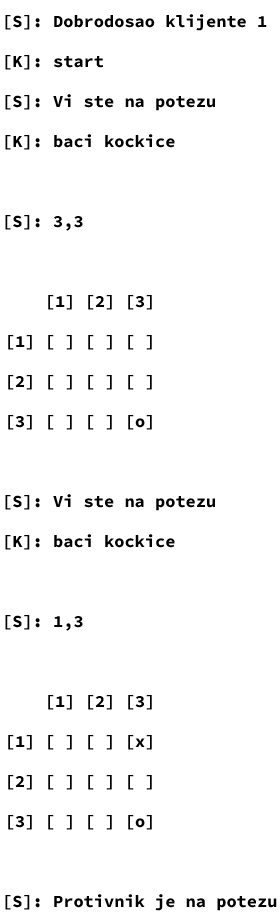
\includegraphics[width=0.25\textwidth]{Slike/DM/DM_Igrac_prvi.png}
    \caption*{Primer komunikacije servera i klijenta koji igra prvi}
    \label{fig:dm_prvi}
\end{figure}

\begin{figure}[H]
    \centering
    
\includegraphics[width=0.25\textwidth]{Slike/DM/DM_Igrac_drugi.png}
    \caption*{Primer komunikacije servera i klijenta koji igra drugi}
    \label{fig:dm_drugi}
\end{figure}

\subsubsection{Primer 2 - Potapanje brodica}

\large{1. Opis zadatka}
\normalsize

Napraviti Client-Server aplikaciju koja će komunicirati na TCP portu X (gde je $X = broj\ indeksa / 24 + 2000)$ i omogućavati klijentima da igraju igru potapanja brodova.

\large{2. Opis igre}
\normalsize

Ovo je popularna i zabavna igra za dva igrača. Cilj igre je potopiti sve brodove protivničke mornarice. Ova igra se pojavljivala na nekolicini takmičenja, uključujući Svetsko takmičenje u slagalicama, i magazinima o slagalicama, kao što je magazin Games.

Igra se na tabli veličine $9\times9$, vrste su označene slovima abecede A-J, dok su kolone označene brojevima 1-9. Pre nego što počne igra, svaki igrač tajno postavi brodove nasvojoj glavnoj tabli. Svaki igrač ima 5 tipova brodova koje raspoređuje na svojoj 9x9 tabli.Veličine brodova su: $1\times5$, $1\times4$, $1\times3$, $1\times2$, $1\times1$. Igrači imaju po dva broda dimenzija $1\times1$ i $1\times2$ i po jedan svih ostalih dimenzija, koje postavljaju na tablu u bilo kojoj orijentaciji ($1\times5$ ili $5\times1$). Sva polja koja zauzima brod moraju biti poravnata duž jedne linije, orijentisana horizontalno ili vertikalno. Brodovi se mogu dodirivati, ali se ne mogu preklapati, tj. na jednom polju se može nalaziti samo jedan brod, kao što je prikazano na slici. Svaki igračdobija isti broj i vrstu brodova.

\begin{figure}[H]
    \centering
    
\includegraphics[width=0.5\textwidth]{Slike/PTP/Dozvoljene pozicije.png}
    \caption*{Primer dozvoljene postavke brodova}
    \label{fig:dozvoljene_postavke}
\end{figure}

\newpage
\large{3. Specifikacija zadatka}
\normalsize

\textbf{Faza I}

Aplikacija treba da podržava konekciju sa dva klijenta koji će uspostavljati komunikaciju sa serverom i predstavljati se kao igrač1 i igrač2. Nakon pokretanja aplikacije i uspešne konekcije sa serverom, klijent započinje igru porukom “start” koju šalje serveru. Server nakon povezivanja prvog klijenta i prijema njegove poruke za početak igre čeka da se konektuje i drugi igrač, a zatim obojicu obaveštava da igra može da počne.

Klijent po prijemu poruke odgovara sa “popuni” i započinje raspoređivanje svojih brodovana svojoj tabli. Popunjavanje se izvršava na sledeći način:

Klijentu se ispisuje poruka o dostupnim brodovima koja će na početku izgledati ovako:

$$[S]:\ {1\times5:\ 1,\ 1\times4:\ 1,\ 1\times3:\ 1,\ 1\times2:\ 2,\ 1\times1:\ 2}$$

Ispod toga se iscrtava tabla (matrica) kao na \textbf{slici 1}:

\begin{figure}[H]
    \centering
    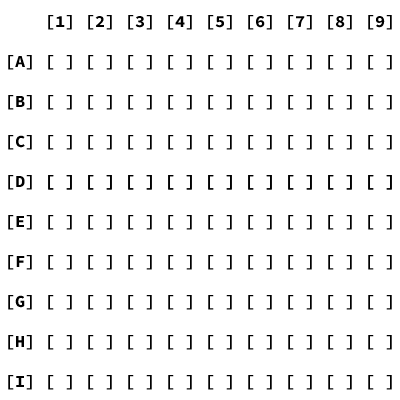
\includegraphics[width=0.5\textwidth]{Slike/PTP/PTP_Pocetak.png}
    \caption*{Slika 1}
    \label{fig:ptp_pocetak}
\end{figure}

Klijent unosi onoliko koordinata kolika je dužina broda ($1\times3$ zahteva 3 koordinate) u formatu {A,1 A, 2 A, 3} gde “A” predstavlja red, dok su brojevi 1, 2 i 3 kolone koje brod zauzima. Brod je potrebno iscrtati na tabeli tako što se polja koja zauzimaju popune znakom “o” i tabela se prikazuje klijentu (videti sliku 2). Kada klijent postavi sve brodove, serveru se prosleđuje tabela u formatu po želji. Server čuva tabele i čeka da oba igrača završe popunjavanje, a zatim ih obaveštava o početku sledeće faze igre.

\begin{figure}[H]
    \centering
    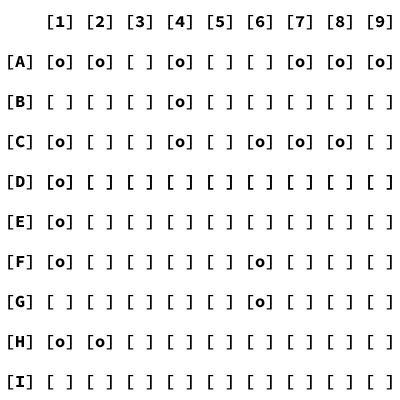
\includegraphics[width=0.5\textwidth]{Slike/PTP/PTP_Postavka.png}
    \caption*{Slika 2}
    \label{fig:ptp_postavka}
\end{figure}

\textbf{Faza II}

U ovoj fazi igrači napadaju i potapaju neprijateljske brodove. Klijent bira polje koje napada u formatu {E,6} i šalje poruku serveru. Server proverava da li se na tom polju nalazi neprijateljski brod ili ne, u zavisnosti od toga vraća “pogodak” ili “promašaj”. Igra traje dok igrač ne potopi sve brodove.

Pobednik je onaj koji potopi suigračeve brodove u manjem broju pokušaja. Klijenti igraju igru nezavisno jedan od drugog (ne postoje potezi). Nakon potapanja svih brodova klijent dobija poruku o svom skoru i obaveštenje da je završio igru.

Nakon kraja igre, protivnik može poslati poruku “status” kojom proverava da li je igra završena i ko je pobedio.

Napomena: sva komunikacija se dešava između klijenta i servera, igrači ne znaju ništa jedan o drugom, osim informacije ko je pobedio nakon poslate poruke „status“.

\begin{figure}[H]
    \centering
    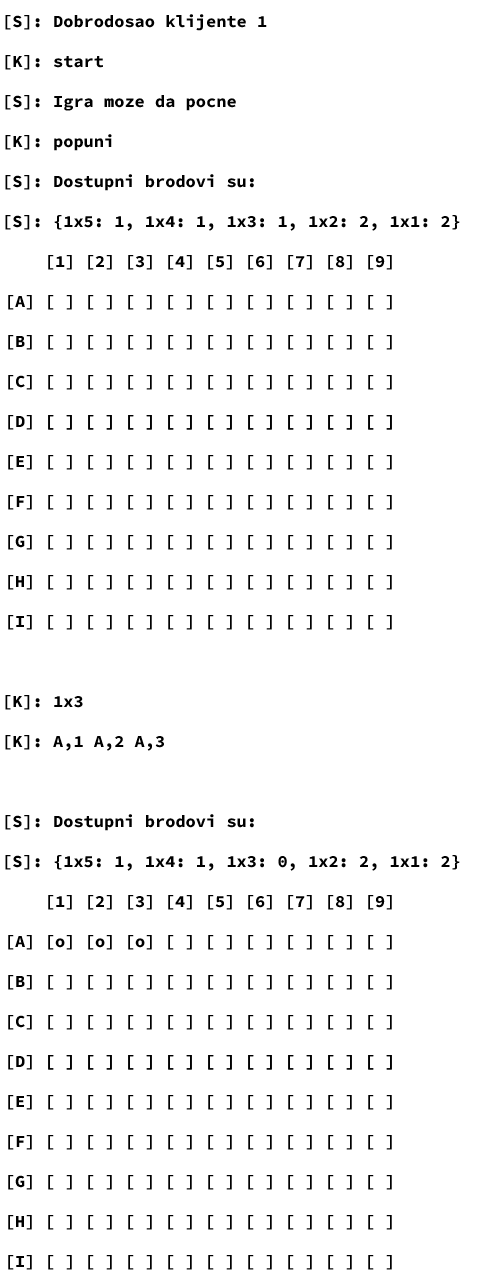
\includegraphics[width=0.5\textwidth]{Slike/PTP/PTP_Primer_komunikacije.png}
    \caption*{Primer postavke brodova}
    \label{fig:ptp_primer_postavke}
\end{figure}

Nakon raspodele svih brodova klijent šalje serveru metu i server mu vraća trenutan izgled table:

\begin{figure}[H]
    \centering
    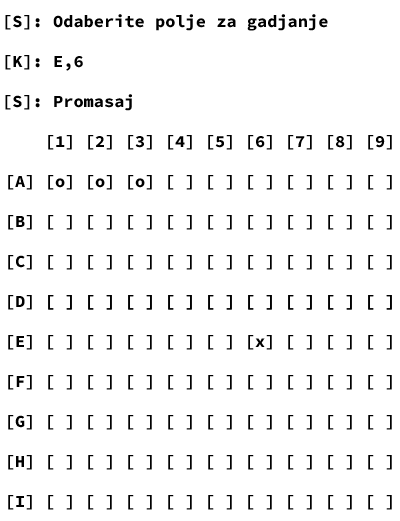
\includegraphics[width=0.5\textwidth]{Slike/PTP/PTP_Promasaj.png}
    \caption*{Primer promasaja}
    \label{fig:ptp_promasaj}
\end{figure}

\begin{figure}[H]
    \centering
    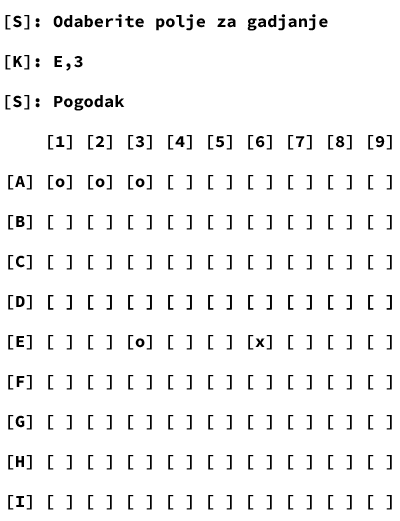
\includegraphics[width=0.5\textwidth]{Slike/PTP/PTP_Pogodak.png}
    \caption*{Primer pogodka}
    \label{fig:ptp_pogodak}
\end{figure}

Po završetku igre server obaveštava korisnika o kraju:

\begin{figure}[H]
    \centering
    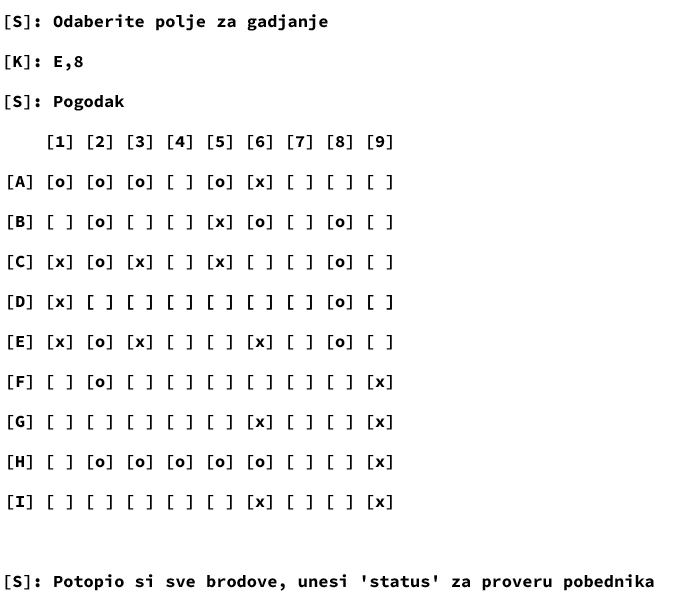
\includegraphics[width=0.8\textwidth]{Slike/PTP/PTP_Pobeda.png}
    \label{fig:ptp_pobeda}
\end{figure}

Provera statusa (moguće je da igra još uvek traje za drugog korisnika ili server ispisuje pobednika):

\begin{figure}[H]
    \centering
    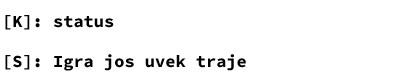
\includegraphics[width=0.5\textwidth]{Slike/PTP/PTP_Status.png}
    \label{fig:ptp_status}
\end{figure}

\subsubsection{Primer 3 - Šifrovana komunikacija}

\large{1. Opis zadatka}
\normalsize

Napraviti Client-Server aplikaciju koja će komunicirati na TCP portu X (gde je $X = broj\ indeksa/24 + 2000$) i omogućavati klijentima šifrovanu komunikaciju koristeći Vigenere tablu sa ključem.

\large{2. Opis šifrovanja}
\normalsize

Vigenere tabla se koristi u šifrovanju poruka pomoću Vigenere šifre. Sastoji se od kvadratne tabele sa 26 redova i 26 kolona, gde svaki red sadrži slova engleskog alfabeta pomerenog za jedno mesto u odnosu na prethodni red. Vigenere tabla sa ključem dodaje kompleksnost tako što se u prvom redu prvo stavljaju sva slova iz ključa, pa tek ostatat alfabeta bez tih slova. 

Da biste šifrovali poruku, prvo odaberete ključnu reč koja se ponavlja do dužine originalne poruke. Ukoliko je ključna reč kraća od originalne poruke, ključna reč se ponavlja sve dok ne dostigne dužinu originalne poruke (Ingorisaći bele i specijalne karaktere), a ukoliko je duža od originalne poruke onda se preseca. Svako slovo u poruci se zatim šifruje kombinovanjem sa odgovarajućim slovom ključne reči korišćenjem tabele: pronađete red koji odgovara slovu ključne reči i kolonu koja odgovara slovu originalne poruke. Slovo na preseku reda i kolone je šifrovano slovo. Dekodiranje se vrši obrnutim procesom koristeći istu tabelu i ključnu reč.

\begin{figure}[H]
    \centering
    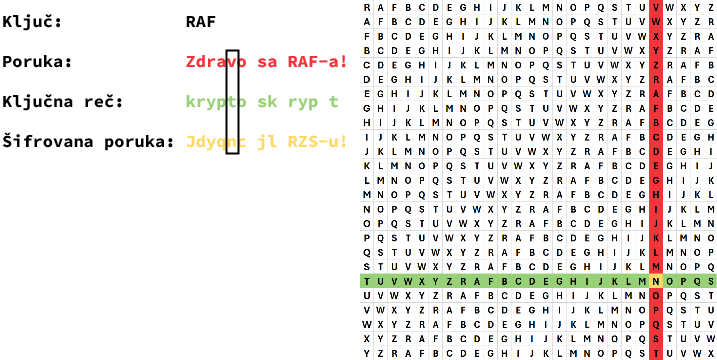
\includegraphics[width=0.85\textwidth]{Slike/VTB/VTB_Sifrovanje.png}
    \caption*{Primer šifrovanja koristeći Vigenere tabelu sa ključem "RAF"}
    \label{fig:vtb_primer}
\end{figure}

\large{3. Specifikacija zadatka}
\normalsize

Aplikacija treba da podrži konekciju \textbf{maksimalno} 2 klijenta. Nakon početka aplikacije, komunikacija kreće tek kada oba igrača kažu start. Pri početku, klijent 1 klijentu 2 šalje ključ i ključnu reč. Oba klijenta generišu alpfabet prema ključu i svu dalju enkripciju i dekripciju rade prema generisanoj Vigenere tabeli i ključnoj reči. Klijent 1 sada šalje poruku klijentu 2. Klijent 2 dešifruje i ispisuje poruku, nakon čega uzvraća šifrovanu poruku. Komunikacija se obavlja sve dok jedan od klijenata ne napiše "!KRAJ!".

\begin{figure}[H]
    \centering
    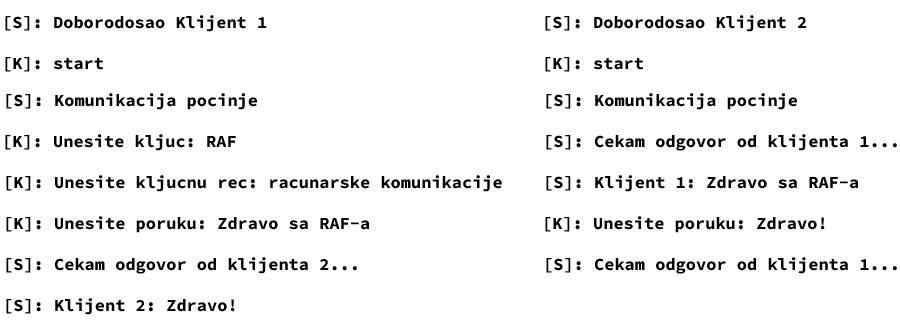
\includegraphics[width=0.85\textwidth]{Slike/VTB/VTB_Primer_komunikacije.png}
    \caption*{Primer komunikacije}
    \label{fig:vtb_primer_komunikacije}
\end{figure}

\subsubsection{Primer 4 - Iks Oks}

\large{1. Opis zadatka}
\normalsize

Napraviti Client-Server aplikaciju koja će komunicirati na TCP portu X (gde je $X = broj\ indeksa/24 + 2000$) i omogućavati klijentima da igraju igru iks-oks.

\large{2. Opis igre}
\normalsize

Iks-oks je igra za dva igrača koja koristi kockice i tablu sa $3\times3$ polja. Igrači neizmenično postavljaju znakove X (Igrač koji ima prvi potez) ili O na tablu sve dok ne postave znakove na tri uzastopna mesta po redovima, kolonama ili dijagonalama. Ukoliko su sva polja popunjena a ni jedan igrač nije ostvario uslov za pobedu, igra je nerešena. Nakon kraja igre može se desiti revanš ukoliko oba igrača žele.

\large{3. Specifikacija zadatka}
\normalsize

Aplikacija treba da podrži konekciju \textbf{maksimalno} 2 klijenta. Nakon početka aplikacije klijent 1 će predstavljati igrača 1 (Igrač 1 ima prvi potez). Igra počinje kada oba klijenta pošalju poruku "start". Nakon poslate poruke, klijent čeka povratnu poruku od servera koja potvrđuje početak igre. Nakon početka igre, server obaveštava klijenta koji je njegov simbol, X ako je igrač 1 a O ako je igrač 2. Na početku svake runde server klijentu šalje trenutno stanje table. Klijent bira polje na kom polju želi da postavi znak u formatu $[i,j]$. Server proverava validnost poteza (Nije moguće postavljanje simbola na već popunjeno polje) i validnost poruke. Ukoliko je došlo do greške, server je ispisuje i traži od korisnika da unese opet željeno polje. Po završetku runde server obaveštava klijente ko je pobednik ili da je igra ne rešena, nakon čega im nudi revanš. Klijenti mogu da pošalju D ukoliko žele revanš ili N ako ne žele. Oba klijenta moraju da se slože za revanš nakon čega im se prezentuje prazna tabla i igraju ispočetka, u suprotnom se igra prekida.

\begin{figure}[H]
    \centering
    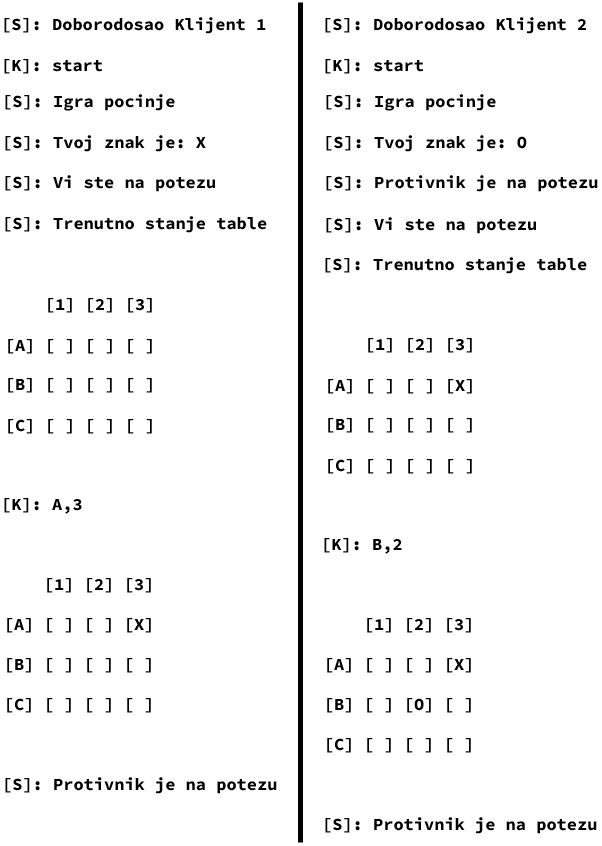
\includegraphics[width=0.5\textwidth]{Slike/XO/XO_Pocetak.png}
    \caption*{Primer pocetka igre. (Levo) Interakcija od strane Klijenta 1. (Desno) Interakcija od strane Klijenta 2}
    \label{fig:xo_pocetak}
\end{figure}